% Autor: Elias Welt
\section{Benutzerprofil (Profile.jsx)}

Die Profilseite gibt dem Nutzer einen Überblick über seine Account-Informationen und ermöglicht grundlegende Kontoverwaltung. Diese Ansicht stellt ein einfaches, aber effektives Muster zum Anzeigen und Aktualisieren von Benutzerdaten dar und ist eine weitere Demostration der durchgängig einfachen Bedienung und hohen UX von EduShelf
\newline

\begin{figure}[h]
    \centering
    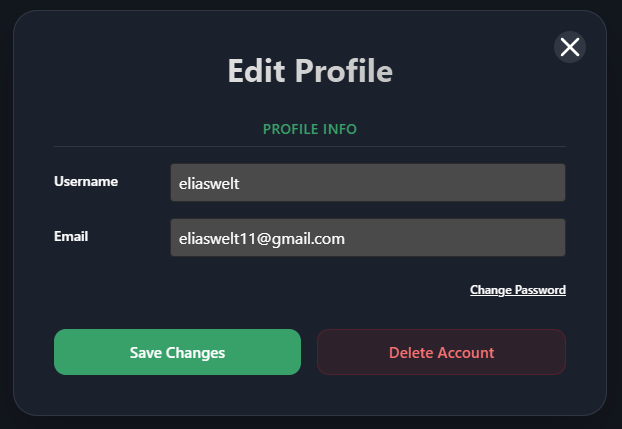
\includegraphics[width=0.6\textwidth]{img/profile-dark-mode}
    \caption{Profilseite von EduShelf im Dark-Mode}
    \label{fig:profile}
\end{figure}

Die Profildaten werden beim Laden der Komponente aus dem \texttt{localStorage} entnommen -- ohne zusätzlichen API-Aufruf. Da die Benutzerdaten (Name, E-Mail, Rollen) bereits beim Login abgerufen und lokal gespeichert wurden, stehen sie sofort zur Verfügung. Dies vermeidet einen unnötigen Netzwerkaufruf und sorgt für eine schnelle Darstellung der Seite.
\newpage
